% Created 2019-08-28 mer. 15:30
% Intended LaTeX compiler: pdflatex
\documentclass[t]{clean-beamer}
\usepackage[utf8]{inputenc}
\usepackage[T1]{fontenc}
\usepackage{graphicx}
\usepackage{grffile}
\usepackage{longtable}
\usepackage{wrapfig}
\usepackage{rotating}
\usepackage[normalem]{ulem}
\usepackage{amsmath}
\usepackage{textcomp}
\usepackage{amssymb}
\usepackage{capt-of}
\usepackage{hyperref}
\usepackage[most]{tcolorbox}
\usepackage{siunitx}
\beamertemplatenavigationsymbolsempty
\addtobeamertemplate{navigation symbols}{}{%
\usebeamerfont{footline}%
\usebeamercolor[fg]{footline}%
\hspace{1em}%
\insertframenumber/\inserttotalframenumber
}
\setbeamertemplate{itemize items}[circle]
\usefonttheme[onlymath]{serif}
\definecolor{mycolor1}{RGB}{79,115,193}
\definecolor{mycolor2}{RGB}{213,91,53}
\usetheme{default}
\author{Dehaeze Thomas}
\date{2019-08-28}
\title{Complementary Filters Shaping\newline Using \(\mathcal{H}_\infty\) Synthesis}
\subtitle{Control System Working Group meeting}
\hypersetup{colorlinks=true}
\hypersetup{
 pdfauthor={Dehaeze Thomas},
 pdftitle={Complementary Filters Shaping\newline Using \(\mathcal{H}_\infty\) Synthesis},
 pdfkeywords={complementary filters, h-infinity, sensor fusion},
 pdfsubject={Complementary Filters Shaping Using H-Infinity Synthesis. Presentation during a Control System Working Group Meeting at LIGO.},
 pdfcreator={Emacs 26.2 (Org mode 9.2.5)},
 pdflang={English}}
\begin{document}

\maketitle

\section{Complementary Filters Shaping}
\label{sec:orgf40a445}
\begin{frame}[label={sec:org644c6eb}]{Sensor Fusion Architecture - Noise Filtering}
\vspace{-1em}
\begin{columns}
\begin{column}{0.45\columnwidth}
\vspace{-1em}
\begin{center}
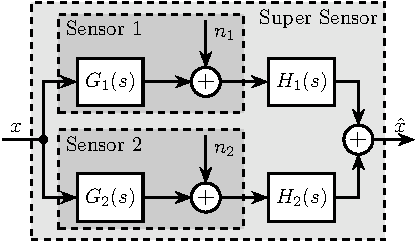
\includegraphics[scale=1,width=1.1\linewidth]{figs/fusion_super_sensor.pdf}
\end{center}
\end{column}

\begin{column}{0.55\columnwidth}
\begin{equation*}
  \hat{x} = \left(G_1 H_1 + G_2 H_2\right) x + H_1 n_1 + H_2 n_2
\end{equation*}

\onslide{\begin{cbox}[Complementary Property]{blue}{}
\begin{equation*}
  H_1(s) + H_2(s) = 1
\end{equation*}
\end{cbox}}\vspace{0.5em}
\end{column}
\end{columns}

\vspace{0.5em}
Let's first consider \textbf{Perfectly Known Sensor Dynamics}:
\begin{equation*}
  G_1(s) = G_2(s) = 1 \Longrightarrow \hat{x} = x + H_1 n_1 + H_2 n_2
\end{equation*}

\onslide{\begin{cbox}[PSD of the Super Sensor's noise]{blue}{ams nodisplayskip}
\begin{equation*}
  \Phi_{\text{ss}} = \left|H_1\right|^2 \Phi_{n_1} + \left|H_2\right|^2 \Phi_{n_2} \Longrightarrow \text{depends on filters' norm}
\end{equation*}
\end{cbox}}\vspace{0.5em}
\end{frame}

\begin{frame}[label={sec:orgaee2e4a}]{Sensor Fusion Architecture - Robustness}
\begin{columns}
\begin{column}{0.5\columnwidth}
\vspace{-2em}
\begin{center}
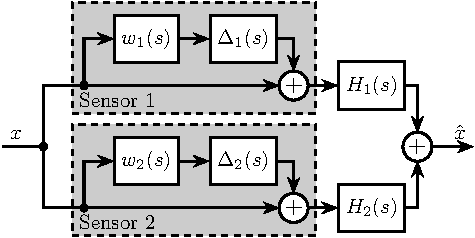
\includegraphics[scale=1,width=1.1\linewidth]{figs/sensor_fusion_dynamic_uncertainty.pdf}
\end{center}
\end{column}

\begin{column}{0.5\columnwidth}
\textbf{Dynamic Uncertainty}:
\begin{gather*}
  G_i^\prime(s) = G_i(s) [1 + w_i(s)\Delta_i(s)],\\
  \quad \forall\Delta_i, \|\Delta_i\|_\infty < 1
\end{gather*}

\textbf{Super Sensor Dynamics}:
\begin{equation*}
  \frac{\hat{x}}{x} = 1 + w_1 H_1 \Delta_1 + w_2 H_2 \Delta_2
\end{equation*}
\end{column}
\end{columns}

\onslide{\begin{cbox}[Limit the Super Sensor Dynamic uncertainty]{blue}{}
Design \(H_1(s)\) and \(H_2(s)\) such that:
\begin{equation*}
  \begin{aligned}
                    & \left|w_1 H_1 \Delta_1\right| + \left|w_2 H_2 \Delta_2\right| \le \epsilon \quad \forall\omega,\ \forall \Delta_1, \forall \Delta_2\\
    \Longleftrightarrow & \left|w_1 H_1\right| + \left|w_2 H_2\right| \le \epsilon \quad \forall\omega \\
    \Longrightarrow & \text{ depends on the filters' norm} \\
  \end{aligned}
\end{equation*}
\end{cbox}}\vspace{0.5em}
\end{frame}

\begin{frame}[label={sec:org1c42552}]{Shaping of Complementary Filters using \(\mathcal{H}_\infty\) synthesis}
\vspace{-1em}
\begin{columns}
\begin{column}{0.5\columnwidth}
\onslide{\begin{cbox}[Design Objective]{blue}{ams nodisplayskip}
\begin{gather*}
  H_1(s) + H_2(s) = 1 \\
  |H_1(j\omega)| \le \frac{1}{|W_1(j\omega)|} \quad \forall\omega \\
  |H_2(j\omega)| \le \frac{1}{|W_2(j\omega)|} \quad \forall\omega
\end{gather*}
\end{cbox}}\vspace{0.5em}

\onslide{\begin{cbox}[]{blue}{}
\(W_1(s)\) and \(W_2(s)\) are proper, stable and minimum phase transfer functions
\end{cbox}}\vspace{0.5em}
\end{column}

\begin{column}{0.5\columnwidth}
\vspace{-3em}
\begin{center}
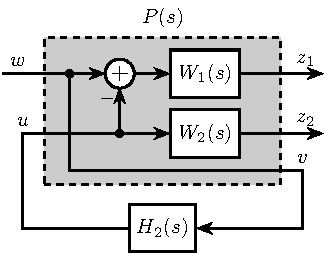
\includegraphics[scale=1,width=\linewidth]{figs/h_infinity_robust_fusion.pdf}
\end{center}

\onslide{\begin{cbox}[\(\mathcal{H}_\infty\) Synthesis]{blue}{}
Find \(H_2(s)\) such that:
\begin{gather*}
  \left\|\begin{matrix} \left[1 - H_2(s)\right] W_1(s) \\ H_2(s) W_2(s) \end{matrix}\right\|_\infty \le 1 \\
  H_1(s) \triangleq 1 - H_2(s)
\end{gather*}
\end{cbox}}\vspace{0.5em}
\end{column}
\end{columns}
\end{frame}

\begin{frame}[label={sec:org493a937}]{Validation of the proposed synthesis method}
\begin{center}
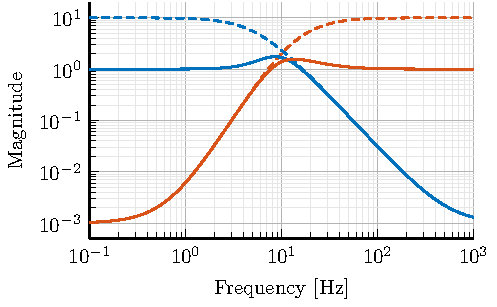
\includegraphics[scale=1,width=0.85\linewidth]{figs/hinf_synthesis_results.pdf}
\end{center}
\end{frame}

\begin{frame}[label={sec:orga95f64f}]{Complementary Filters Used at LIGO - Specifications}
The specification are detailed in \emph{Hua, W., Low frequency vibration isolation and alignment system for advanced LIGO (2005)}

\begin{center}
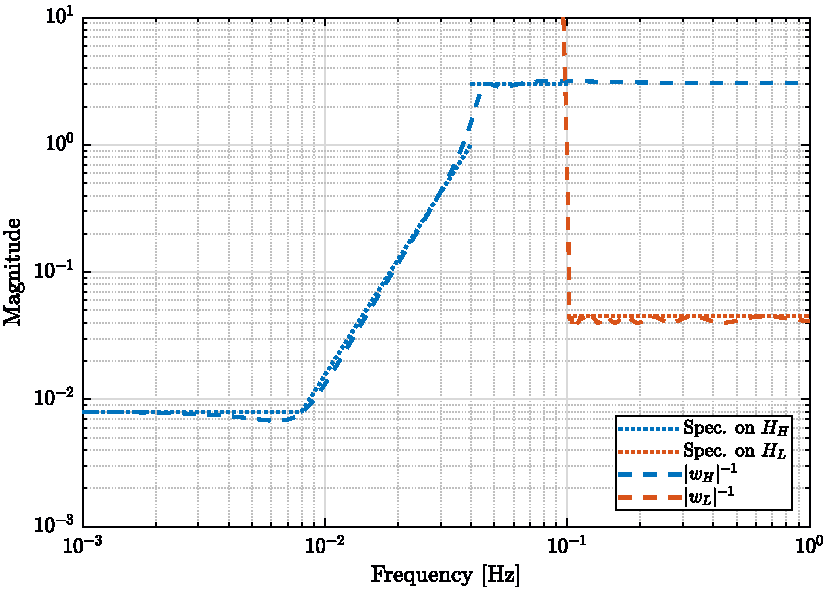
\includegraphics[scale=1,width=0.8\linewidth]{figs/ligo_weights.pdf}
\end{center}

\onslide{\begin{cbox}[Weighting Functions used]{blue}{}
\begin{center}
\begin{tabular}{ll}
\(\tikz[baseline=-0.5ex]{\draw[color=mycolor1, line width=1.5pt](0,0)--(1,0)}\) & Custom Designed \(7^{\text{th}}\) Order Transfer Function\\
\(\tikz[baseline=-0.5ex]{\draw[color=mycolor2, line width=1.5pt](0,0)--(1,0)}\) & Type I Chebyshev Filter of Order \(20\)\\
\end{tabular}
\end{center}
\end{cbox}}\vspace{0.5em}
\end{frame}

\begin{frame}[label={sec:org3e0dbb2}]{\(\mathcal{H}_\infty\) Synthesis - Comparison with LIGO's FIR filters}
\begin{columns}
\begin{column}{0.6\columnwidth}
\vspace{-3em}
\begin{center}
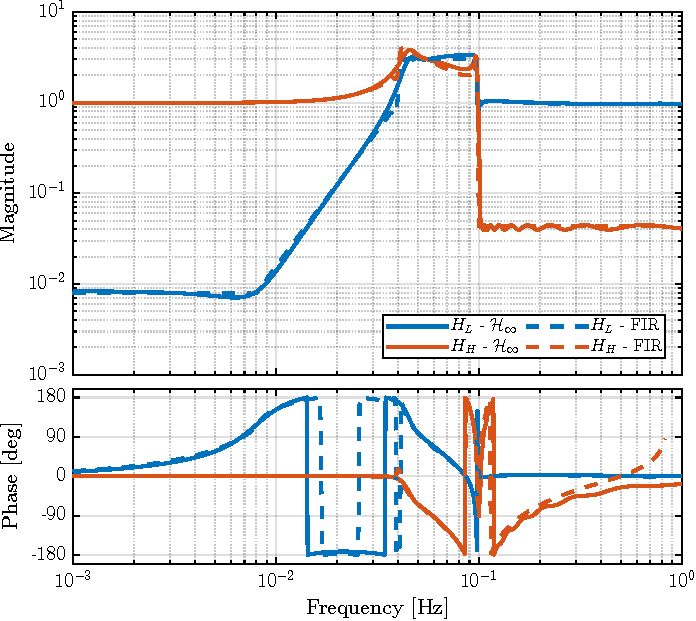
\includegraphics[scale=1,width=1.1\linewidth]{figs/comp_fir_ligo_hinf.pdf}
\end{center}
\end{column}

\begin{column}{0.4\columnwidth}
\begin{itemize}
\item FIR Filters: order 512
\item \(\mathcal{H}_\infty\) Filters: order 27
\end{itemize}

\vspace{1em}

\onslide{\begin{cbox}[]{blue}{}
The paper and all the Matlab Scripts used for the paper are accessible \href{https://tdehaeze.github.io/dehaeze19\_desig\_compl\_filte/}{here}.
\end{cbox}}\vspace{0.5em}
\end{column}
\end{columns}

\onslide{\begin{cbox}[Conclusion]{blue}{}
Specifications: expressed as upper bounds on the filters' norm\\
\(\mathcal{H}_\infty\) Synthesis: easily shape complex complementary filters
\end{cbox}}\vspace{0.5em}
\end{frame}
\end{document}